%\documentclass[a4paper,10pt,hungarian]{report}
%\documentclass[a4paper,10pt,hungarian]{article}
\documentclass[a4paper,10pt]{article}
%a ,,hungarian'' opci� csak a draftcopy csomaghoz kell!
%\usepackage[latin2]{inputenc}
%\usepackage[T1]{fontenc}
%\usepackage[magyar]{babel}
%\usepackage[left=2.5cm,right=2.5cm,top=2cm,bottom=2cm]{geometry}
\usepackage[left=2.5cm,right=2cm,top=2cm,bottom=2cm]{geometry}
\usepackage{indentfirst}
\usepackage{upgreek}
\usepackage{relsize}
\usepackage{hyperref}
\usepackage{ifthen}
\usepackage{scrextend}
\addtokomafont{labelinglabel}{\sffamily}
\usepackage{tikz}
\usetikzlibrary{calc,fit,arrows,positioning}
\sloppy
%\usepackage{graphicx}
%\usepackage{ifthen}
%\usepackage{multicol}
%\usepackage[outline]{draftcopy} %outline,bottom,light,none/first/firsttwo
%\usepacgake{wasysym}
%%%% Don't modify next two line! %%%%
%.PDF.\usepackage{times}
%.PDF.\usepackage[T1]{mathtime}
\frenchspacing
\newcommand{\mypi}{{\larger $\uppi$}}
%\newcommand{\mypi}{{\larger $\pi$}}
\newcommand{\pifs}{\mypi{}fs}
\newcommand{\pifsl}{Pi file system}

%%% TiKZ
\tikzstyle{block} = [draw,fill=yellow!20,dashed,minimum size=2.5cm,inner sep=0.45cm]
\tikzstyle{blocktext} = [text width=2.4cm,align=left]
\tikzstyle{page} = [draw,fill=brown!25,dashed,minimum width=2cm,minimum height=0.8cm,text width=1.6cm,align=left]
\tikzstyle{flash} = [draw,fill=gray!15,inner sep=0.45cm]
% diameter of semicircle used to indicate that two lines are not connected
\def\radius{.7mm} 
\tikzstyle{branch}=[fill,shape=circle,minimum size=3pt,inner sep=0pt]
\makeatletter
\tikzset{
    dot diameter/.store in=\dot@diameter,
    dot diameter=2pt,
    dot spacing/.store in=\dot@spacing,
    dot spacing=8pt,
    dots/.style={
        line width=\dot@diameter,
        line cap=round,
        dash pattern=on 0pt off \dot@spacing
    }
}
\makeatother
% Define layers, otherwise gray blocks will hide pages
\pgfdeclarelayer{background}
\pgfdeclarelayer{background2}
\pgfsetlayers{background,background2,main}
%%% End of TiKZ

\author{Peter Ivanov \textless{}ivanovp@gmail.com\textgreater{}}
\title{\pifsl{} (\pifs{})}
%%
%\usepackage[dvips]{graphicx}

%%

\begin{document}
\maketitle
%\tableofcontents
\section{Introduction}
This file system was developed for embedded systems which use NOR flash as 
storage. 
The development started as teach-myself project and I released the code in 
hope that it will be useful for someone else as well.

NOR flash ICs have very low price nowadays (2017) and can be used
to store files. But there are few problems to consider when designing a file
system:
\begin{itemize}
\item NOR flashes can be programmed (set bits to zero) by pages, but only 
can be erased (set bits to one) in a larger quantity, which are mostly called
block in the datasheets. One page is usually 256 or 512 bytes, one block 
consits of 16, 256, 1024, etc. pages. So typical block sizes are 4 KiB, 
64 KiB, 256 KiB.
\item Blocks can be erased ~10,000--100,000 times. After that data retention is 
not guaranteed. Therefore all blocks should be erased uniformly. This method 
is called wear leveling.
\end{itemize}

\pifs{} can be scaled from 4 Mbit (512 KiB), 256 Mbit (32 MiB), 
theoretically up to 1 Gbit (128 MiB) memory sizes.

\subsection{Features of the \pifs{}}
\begin{itemize}
\item Small memory footprint
\item Files can be opened for update ("r+", "w+", "a+" modes are supported)
\item Size of logical page is user-defined
\item Cache buffer for page (currently only one page is cached)
\item Directory handling
\item Dynamic wear-leveling
\item Static wear-leveling (limited, work-in-progress)
\item User data can be added for files: permissions, owner IDs, etc.
\item At the beginning of flash memory reserved blocks can be defined, which 
are not used by the file system
\end{itemize}

\subsection{Limitations of the \pifs{}}
\begin{itemize}
\item Only one flash chip can be used (one volume is supported)
\item Memory and file system configuration cannot be changed during run-time
\item One directory can only store pre-defined number of files or directories
\item No OS support yet, file system can be used only from one task
\item Incompatible with FAT file system, therefore cannot be used for USB mass
storage devices
\end{itemize}

\section{Definitions, Acronyms and Abbreviations}
\begin{labeling}{File system header} % <--- here goes the longest definition to measure the necessary space
\item[NOR flash] Special type of EEPROMs, which manufactured using NOR gates.

\item[Page] Array of several bytes in the flash memory. Number of bytes is 
power of two, usually 256 or 512 bytes. See \autoref{fig:flash}.

\item[Block] Composed of several pages. Usually a block contain 16, 256 or 1024
pages. See \autoref{fig:flash}.

\item[Erase] Change data bits to one (logical high level). Only a whole block 
can be erased, which means all bits of the block are set to one.

\item[Program] Change data bits to zero (logical low level). Each bit of a page can be programmed individually.

\item[Block address] Index of block in flash memory. Type: pifs\_block\_address\_t

\item[Page address] Index of a page in a block. Type: pifs\_page\_address\_t

\item[Page offset] Index of a byte in a page. Type: pifs\_page\_offset\_t

\item[Data area] Blocks which hold the file's content. See \autoref{fig:flashfs}.

\item[Management area] Blocks which hold the file system's internal
data, how much space is allocated, where are the data pages of files, etc. There are two types of management area: primary (active) management area, secondary (next) management area.
See \autoref{fig:flashfs}.

\item[File system header] First page of active management area contains the
header of file system. It describes address of free space bitmap, entry list,
delta map, wear level list, etc.
Type: pifs\_header\_t, variable: pifs.header.

\item[FSBM] Free space bitmap. It stores information about all pages of flash memory:
1 bit stores whether page is free, 1 bit stores if page is to be released.

\item[Delta page] If content of a file is overwritten and original page
cannot be overwritten because bits should be changed from 0 to 1, delta pages 
are added. When the original page is read from a given address the content of
delta page is provided from a different address.

\item[Map page] Management page which is used to describe data pages of a file.

\item[Entry list] Technically a directory of file system.

\item[Entry] One file or directory in the directory.

\item[TBR] To be released. A page which was used, but now it can erased then 
allocated. If all pages in a block marked TBR, the block can be erased.

\item[Merge] During merge management area is written, blocks are erased, delta pages are resolved and entry list is compacted. The data is copied from primary to secondary management area and the next secondary management area is selected.
\end{labeling}

\begin{figure}[h]
\centering
%%%%%%%%%%%%%%%%%%%%
%%% Flash figure %%%
%%%%%%%%%%%%%%%%%%%%

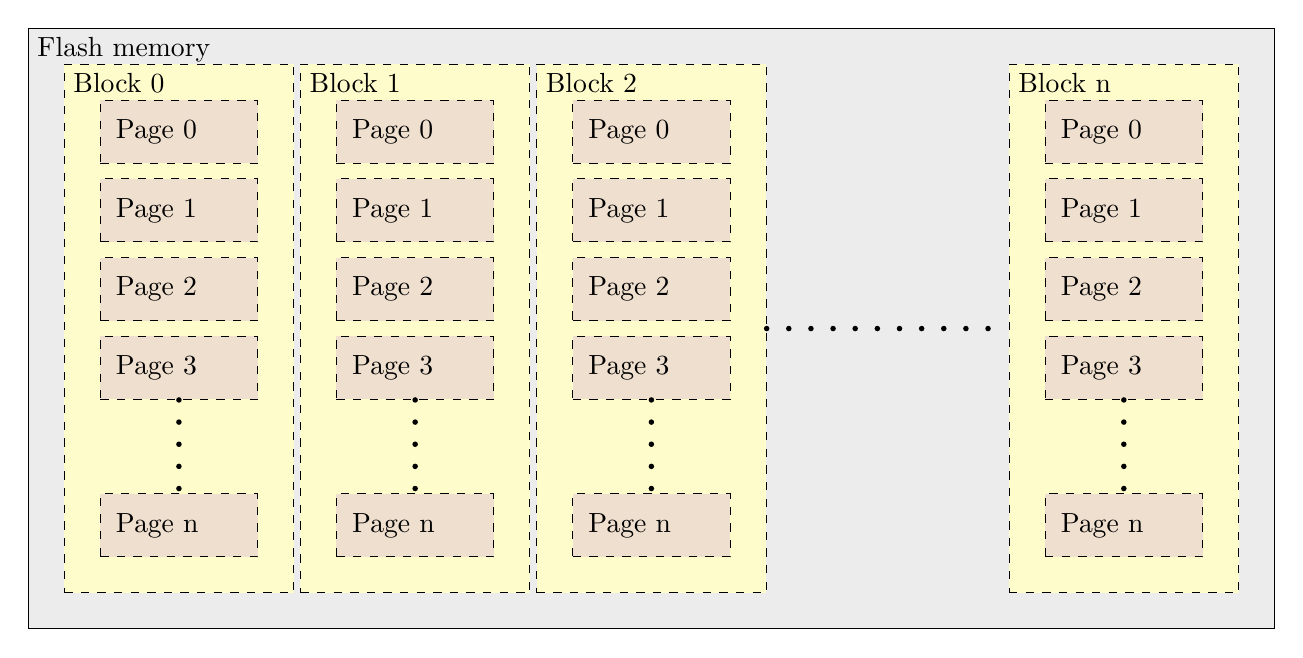
\begin{tikzpicture}[>=latex']
%%% Draw blocks 0..2
\foreach \x in {0,1,2} {
    % Draw pages
    \foreach \y in {0,1,2,3} {
        \node[page] at (\x * 3,-\y) (page\x\y) {Page \y};
    }
    \def\y{5}
    \node[page] at (\x * 3,-\y) (page\x\y) {Page n};
    \draw[dots] (page\x3) -- (page\x\y);
    \begin{pgfonlayer}{background2}
    % Draw block
    \node[fit=(page\x0) (page\x\y), block] (block\x){};
    \node[below right,blocktext] at (block\x.north west) {Block \x};
    \end{pgfonlayer}
}
%%% Draw block n
\def\x{4}
% Draw pages
\foreach \y in {0,1,2,3} {
    \node[page] at (\x * 3,-\y) (page\x\y) {Page \y};
}
\def\y{5}
\node[page] at (\x * 3,-\y) (page\x\y) {Page n};
\draw[dots] (page\x3) -- (page\x\y);
\begin{pgfonlayer}{background2}
% Draw block
\node[fit=(page\x0) (page\x\y), block] (block\x){};
\draw[dots] (block2) -- (block\x);
\node[below right,blocktext] at (block\x.north west) {Block n};
\end{pgfonlayer}

\begin{pgfonlayer}{background}
\node[fit=(block0) (block4),flash] (flash){};
\node[below right] at (flash.north west) {Flash memory};
\end{pgfonlayer}
\end{tikzpicture}

\caption{Flash memory layout}
\label{fig:flash}
\end{figure}

\begin{figure}[h]
\centering
%%%%%%%%%%%%%%%%%%%%%%%
%%% Flash FS figure %%%
%%%%%%%%%%%%%%%%%%%%%%%

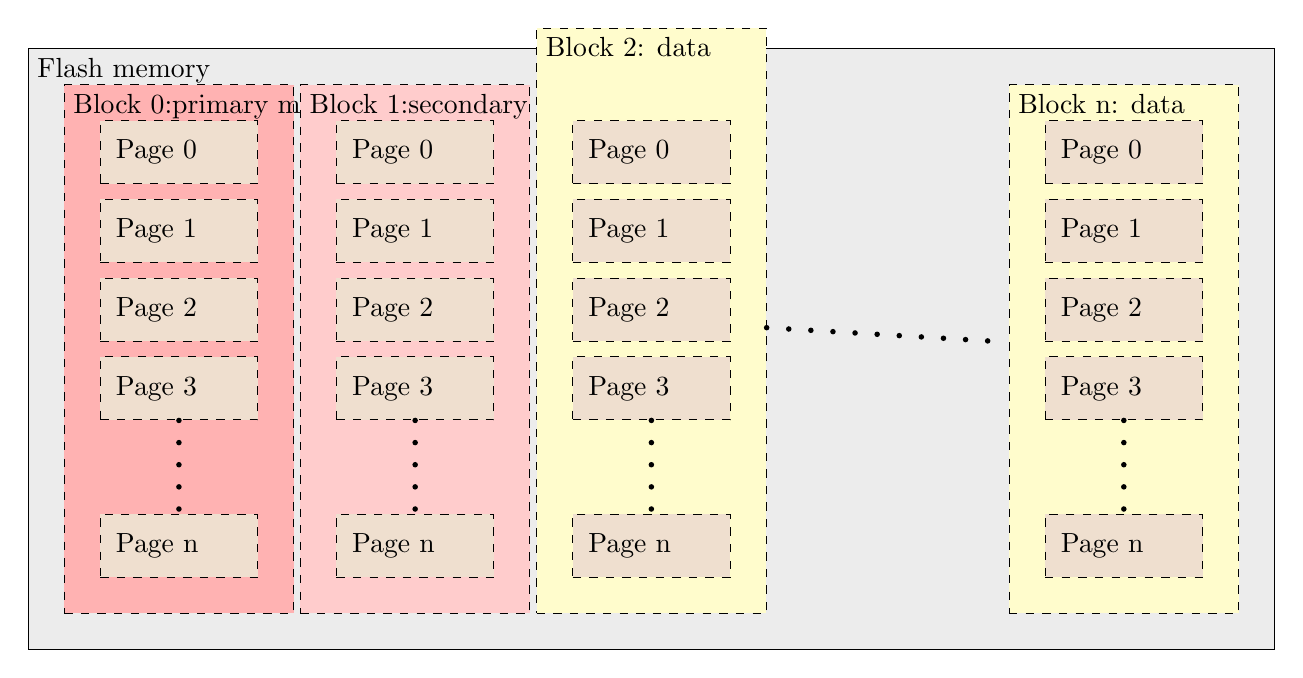
\begin{tikzpicture}[>=latex']
%%% Draw blocks 0..2
\foreach \x in {0,1,2} {
    % Draw pages
    \foreach \y in {-1,0,1,2,3} {
        \ifthenelse{-1 = \y}
        {
            % Invisible!
            \node[draw=none] at (\x * 3,-\y) (page\x\y) {};
        }
        {
            \node[page] at (\x * 3,-\y) (page\x\y) {Page \y};
        }
    }
    \def\y{5}
    \node[page] at (\x * 3,-\y) (page\x\y) {Page n};
    \draw[dots] (page\x3) -- (page\x\y);
    \begin{pgfonlayer}{background2}
    % Draw block
    \ifthenelse{0 = \x \OR 1 = \x}
    {
        \ifthenelse{0 = \x}
        {
            % primary management
            \node[fit=(page\x0) (page\x\y), block,fill=red!30] (block\x){};
            \node[below right] at (block\x.north west) {\hbox{Block \x: \newline
            primary management}};
        }
        {
            % secondary management
            \node[fit=(page\x0) (page\x\y), block,fill=red!20] (block\x){};
            \node[below right] at (block\x.north west) {\hbox{Block \x: \newline
            secondary management}};
        }
    }
    {
        % data
        \node[fit=(page\x-1) (page\x\y), block] (block\x){};
        \node[below right] at (block\x.north west) {Block \x: data};
    }

    \end{pgfonlayer}
}
%%% Draw block n
\def\x{4}
% Draw pages
\foreach \y in {-1,0,1,2,3} {
    \ifthenelse{-1 = \y}
    {
        % Invisible!
        \node[draw=none] at (\x * 3,-\y) (page\x\y) {};
    }
    {
        \node[page] at (\x * 3,-\y) (page\x\y) {Page \y};
    }
}
\def\y{5}
\node[page] at (\x * 3,-\y) (page\x\y) {Page n};
\draw[dots] (page\x3) -- (page\x\y);
\begin{pgfonlayer}{background2}
% Draw block
\node[fit=(page\x0) (page\x\y), block] (block\x){};
\draw[dots] (block2) -- (block\x);
\node[below right] at (block\x.north west) {Block n: data};
\end{pgfonlayer}

\begin{pgfonlayer}{background}
\node[fit=(block0) (block4),flash] (flash){};
\node[below right] at (flash.north west) {Flash memory};
\end{pgfonlayer}
\end{tikzpicture}
            
%\footnotetext{Primary management block}
%\footnotetext{Secondary management block}


\caption{Flash memory layout when \pifs{} installed}
\label{fig:flashfs}
\end{figure}

\end{document}
